\documentclass[../main.tex]{subfiles}
\begin{document}

\subsection{Evaluation with wallets dataset}

\figref{hist_wallets}

\begin{figure*}[ht!]
  \centering
  \includegraphics[clip,trim={14 24 28 25},width=.24\textwidth]{../../ethereum-contract-similarity/runs/wallets/out/all hist raw jump.png}
  \includegraphics[clip,trim={14 24 28 25},width=.24\textwidth]{../../ethereum-contract-similarity/runs/wallets/out/all hist skeletons jump.png}
  \includegraphics[clip,trim={14 24 28 25},width=.24\textwidth]{../../ethereum-contract-similarity/runs/wallets/out/all hist fstSecSkel jump.png}
  \includegraphics[clip,trim={14 24 28 25},width=.24\textwidth]{../../ethereum-contract-similarity/runs/wallets/out/all hist fStat0 jump.png}\\

  \includegraphics[clip,trim={14 24 28 25},width=.24\textwidth]{../../ethereum-contract-similarity/runs/wallets/out/all hist raw ssdeep.png}
  \includegraphics[clip,trim={14 24 28 25},width=.24\textwidth]{../../ethereum-contract-similarity/runs/wallets/out/all hist skeletons ssdeep.png}
  \includegraphics[clip,trim={14 24 28 25},width=.24\textwidth]{../../ethereum-contract-similarity/runs/wallets/out/all hist fstSecSkel ssdeep.png}
  \includegraphics[clip,trim={14 24 28 25},width=.24\textwidth]{../../ethereum-contract-similarity/runs/wallets/out/all hist fStat0 ssdeep.png}\\

  \includegraphics[clip,trim={14 24 28 25},width=.24\textwidth]{../../ethereum-contract-similarity/runs/wallets/out/all hist raw ppdeep_mod.png}
  \includegraphics[clip,trim={14 24 28 25},width=.24\textwidth]{../../ethereum-contract-similarity/runs/wallets/out/all hist skeletons ppdeep_mod.png}
  \includegraphics[clip,trim={14 24 28 25},width=.24\textwidth]{../../ethereum-contract-similarity/runs/wallets/out/all hist fstSecSkel ppdeep_mod.png}
  \includegraphics[clip,trim={14 24 28 25},width=.24\textwidth]{../../ethereum-contract-similarity/runs/wallets/out/all hist fStat0 ppdeep_mod.png}\\

  \includegraphics[clip,trim={14 24 28 25},width=.24\textwidth]{../../ethereum-contract-similarity/runs/wallets/out/all hist raw bz.png}
  \includegraphics[clip,trim={14 24 28 25},width=.24\textwidth]{../../ethereum-contract-similarity/runs/wallets/out/all hist skeletons bz.png}
  \includegraphics[clip,trim={14 24 28 25},width=.24\textwidth]{../../ethereum-contract-similarity/runs/wallets/out/all hist fstSecSkel bz.png}
  \includegraphics[clip,trim={14 24 28 25},width=.24\textwidth]{../../ethereum-contract-similarity/runs/wallets/out/all hist fStat0 bz.png}

  \caption{wallets}
  \label{fig:hist_wallets}
\end{figure*}

\subsection{solc-version-testset}
ABI v2 moves the majority of the interface code from the start to the end of the code compared to v1.

Optimization changes the how the ABI jump table is realized, solely causing significant changes for domain independent similarity measures.

Optimizations with high runs settings lead to a heavy reliance on storage operations, and causes a dramatically increase in overall code length.

Version changes are comparably smaller, but the default ABI encoding changed from v1 to v2 with solc version 0.8.0.

\todo{how do I know this?}

\subsection{jumpHash}
Considering its simplicity it performs surprisingly well in separating contracts from different groups, partially due to the fact that the number of JUMPI opcodes has a very high f-statistic value.

It correlates strongly with NCD, wich seams to be more robust to optimization changes, but comparisons take 30 times longer and jumpHash separates groups more sharply.

\todo{sharply?}
\todo{How do I know this?}

The nativ Levenshtein implementation used for comparison is the fastest out of all hash similarities used in this work. Only Jaccard applied to the much shorter Fourbyte signature sets is faster.

\todo{investigate clusters within groups}

\subsection{Bytebag}
Combined with skeletonization and opcode filtering Bytebag performs better than ssdeep in some scenarios.

\subsection{LZJD parameters}

\tblref{lz_sep}

\begin{table}[ht!]
  \centering
  \csvreader[
    tabular=r|ll,
    table head= & Measure & Separation\\\hline,
    head to column names]{csv/lzjd_all_separation.csv}{}{\thecsvrow & \measure & \separation}

  \caption{separations}
  \label{tbl:lz_sep}
\end{table}

%\csvautotabular{../csv/lzjd_all_separation.csv}

\subsection{ssdeep variants}

\subsection{F-Stat filter}


\subsection{Solc Versions clustered with byteBagJaccard}

\subsubsection{Data}

Nine Solidity source files compiled with 4 solc versions (5, 6, 7, 8) times three optimization
settings (no optimization, runs = 1, runs = 999999).

Necessary changes where made to the source code to ensure compatibility with the different solc
version without altering the function of the contracts.

The runtime codes where segmented and the first segments skeletonized.

\subsubsection{Similarity}
Similarity was calculated via byteBagJaccard after filtering the op-codes with an opcode filter.

\underline{Opcode filter}
\begin{lstlisting}[style=pymd]
(OP.is_log() or OP.is_storage() or OP.is_sys_op() or OP.is_env_info()
  or OP.is_block_info() or OP == opcodes.SHA3 or OP == opcodes.GAS)
\end{lstlisting}

\subsubsection{Clustering}
Clustering was done with Gephi (0.9.2), see figure for settings.

\subsubsection{Observation}
The clustering algo first mixed a few similar contracts into one blob, with a little manual help
it formed cohesive clusters \figref{solc_bytebag_cluster}.

Noticeable is that the Synthetix codes without optimization from all 4 solc versions form a cluster
separate from the other Synthetix code.

\begin{figure*}[ht!]
  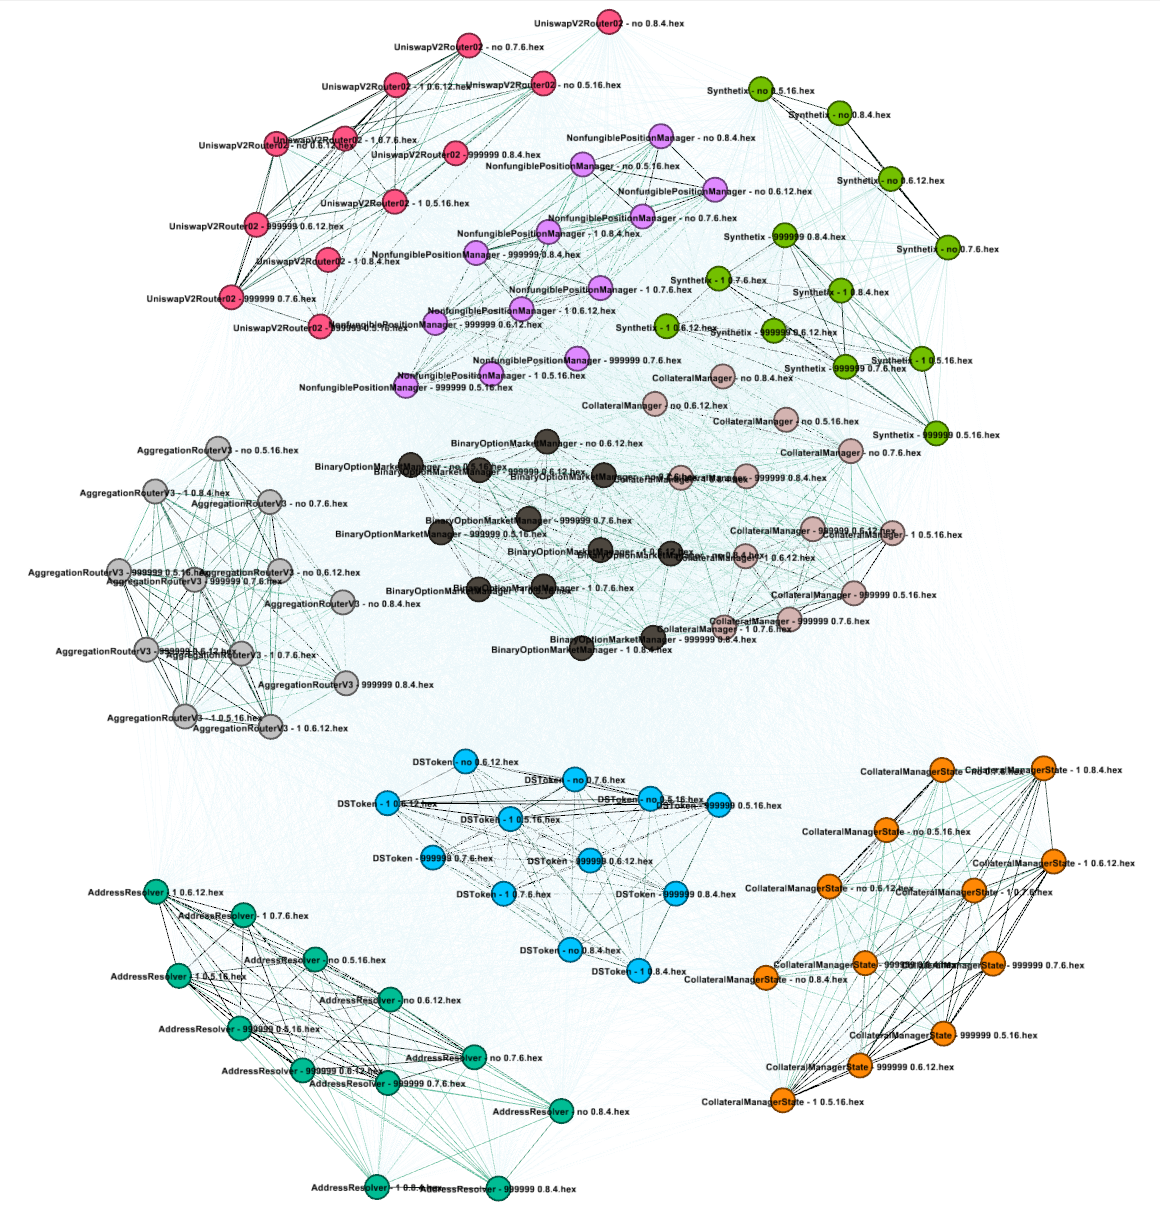
\includegraphics[width=\linewidth]{clustering_result_many_solc_versions_byteBag_significant_only_2021-06-06_163755.png}
  \caption{bytebag cluster with force-atlas}
  \label{fig:solc_bytebag_cluster}
\end{figure*}

\subsubsection{Analysis}
When comparing the frequency of the op-codes in `Synthetix - no 0.8.4.hex` and
`Synthetix - 999999 0.8.4.hex` the following 7 op-codes show the highest change.

\begin{table}[ht!]
  \centering
  \csvreader[
    tabular=rrlrrr,
    table head= dec & hex & op-code & no 0.8.4 & 999999 0.8.4 & diff\\\hline,
    head to column names]{csv/opt_diff.csv}{}{%
      \csvcoli & \texttt{\csvcolii} & \csvcoliii & \csvcoliv & \csvcolv & \csvcolvi}
  \caption{optimization differences}
  \label{tbl:opt_diff}
\end{table}

\begin{ul}
  \item `54 0x36 CALLDATASIZE` is the most consistent across solc versions and optimization settings.
  \item `59 0x3B EXTCODESIZE` is also very consistent. [csv]
  \item `90 0x5A GAS` has a high absolute difference between the Synthetix contracts but it has higher differences across contracts.
\end{ul}

\subsubsection{Interpretation}
The `RETURN` code should definitely be filtered out since optimization drastically reduces its prevalence.

Optimization options change the codes more than solc version changes.


\end{document}
